\documentclass[11pt]{article}
\usepackage[utf8]{inputenc}	% Para caracteres en español
\usepackage{amsmath,amsthm,amsfonts,amssymb,amscd}
\usepackage{multirow,booktabs}
\usepackage[table]{xcolor}
\usepackage{fullpage}
\usepackage{lastpage}
\usepackage{enumitem}
\usepackage{fancyhdr}
\usepackage{mathrsfs}
\usepackage{wrapfig}
\usepackage{setspace}
\usepackage{calc}
\usepackage{multicol}
\usepackage{cancel}
\usepackage[retainorgcmds]{IEEEtrantools}
\usepackage[margin=3cm]{geometry}
\usepackage{amsmath}
\newlength{\tabcont}
\setlength{\parindent}{0.0in}
\setlength{\parskip}{0.05in}
\usepackage{empheq}
\usepackage{framed}
\usepackage[most]{tcolorbox}
\usepackage{xcolor}
\colorlet{shadecolor}{orange!15}
\parindent 0in
\parskip 12pt
\geometry{margin=1in, headsep=0.25in}
\theoremstyle{definition}
\newtheorem{defn}{Definition}
\newtheorem{reg}{Rule}
\newtheorem{exer}{Exercise}
\newtheorem{note}{Note}
\begin{document}
\setcounter{section}{0}
\title{Spin Echoes}

\thispagestyle{empty}

\begin{center}
{\LARGE \bf Spin Echoes}\\
{\large Biophysics 03-230}\\
Nikolai Mickevicius, Ph.D.\\
11$^\text{th}$ September, 2025
\end{center}

\section{Background}

\subsection{Relaxation Review}

The rate at which longitudinal magnetization \emph{recovers} toward an equilibrium magnetization $M_0$ after being converted into transverse magnetization is described by the time constant $T_1$, where $M_z(t) = M_0 \left(1 - e^{-t/T_1} \right)$. The rate at which transverse magnetization \emph{decays} is described by $T_2$ as $M_{\perp}(t) = M_{\perp,0} e^{-t/T_2}$.

\subsection{Larmor Equation and Phase Review}

Once again, we will rely heavily on the Larmor equation, where $\omega = \gamma B$, and following an RF excitation, spins will accumulate phase as a function of the time since excitation $T$ as $\phi = \gamma B T$. In general, we examine the signal phase relative to the nominal frequency of our RF transmitter and receiver, so a more accurate relationship is given by $\phi = \gamma \cdot \Delta B \cdot T$, where $\Delta B$ is a deviation from the nominal field strength of the scanner given in units of Tesla. 

\subsection{Vector Representation of Magnetization}

The magnetization in each voxel is parameterized by its longitudinal (i.e., aligned with the static field) and transverse (i.e., perpendicular to the static field) components. Since the latter has a phase as described above, separate $x$ and $y$ components are needed to fully describe the magnetization. In vector form, the magnetization can be described in real-valued Cartesian coordinates as 
\begin{equation}
    \mathbf{M} = \begin{bmatrix}
        M_x\\
        M_y\\
        M_z
    \end{bmatrix}.
\end{equation}
Additionally, the some mathematics of the Bloch equations are more easily described if we perform a coordinate transformation with a similarity matrix $\mathbf{S}$ such that we use complex numbers to describe the transverse magnetization as a complex conjugate pair:
\begin{equation}
\begin{bmatrix}
        M_x\\
        M_y\\
        M_z
    \end{bmatrix} \underset{\mathbf{S}^{-1}}{\stackrel{\mathbf{S}}{\rightleftharpoons}} \begin{bmatrix}
        M_x + iM_y\\
        M_x - iM_y\\
        M_z
    \end{bmatrix},
\end{equation}
where 
\begin{equation}
    \mathbf{S} = \begin{bmatrix}
        1 & i & 0 \\
        1 & -i & 0 \\
        0 & 0 & 1
    \end{bmatrix}.
\end{equation}

\subsection{Matrix-Vector Representation of Free Precession}

Using the Cartesian representation of magnetization, free precession (i.e., accumulation of phase in the absence of RF) can be described as a rotation matrix $\mathbf{R}_z$ times the magnetization: 

\begin{equation}
    \mathbf{M}^\prime = 
    \begin{bmatrix}
        M_x^\prime \\
        M_y^\prime \\
        M_z^\prime
    \end{bmatrix} = 
    \mathbf{R}_z \mathbf{M} = 
    \begin{bmatrix}
        \cos \phi & -\sin \phi & 0 \\
        \sin \phi & \cos \phi & 0 \\
        0 & 0 & 1
    \end{bmatrix}
    \begin{bmatrix}
        M_x\\
        M_y\\
        M_z
    \end{bmatrix} = 
    \begin{bmatrix}
        M_x \cos \phi - My \sin \phi \\
        M_x \sin \phi + M_y \cos \phi \\
        M_z
    \end{bmatrix}
\end{equation}

\subsection{Matrix-Vector Representation of RF Pulses}

Similarly as above, rotations about the $x$ and $y$ axes due to RF pulses can be described using rotation matrices. The angle about which the magnetization is rotated along each direction is given by the flip angles $\phi_x = \gamma B_{1,x} T$ and $\phi_y = \gamma B_{1,y} T$.

\begin{equation}
    \mathbf{M}^\prime = 
    \begin{bmatrix}
        M_x^\prime \\
        M_y^\prime \\
        M_z^\prime
    \end{bmatrix} = 
    \mathbf{R}_x \mathbf{R}_y \mathbf{M} = 
    \begin{bmatrix}
        1 & 0 & 0 \\
        0 & \cos \phi_x & -\sin \phi_x \\
        0 & \sin \phi_x & \cos \phi_x
    \end{bmatrix}
    \begin{bmatrix}
        \cos \phi_y & 0 & \sin \phi_y \\
        0 & 1 & 0 \\
        -\sin \phi_y & 0 & \cos \phi_y
    \end{bmatrix}
    \begin{bmatrix}
        M_x\\
        M_y\\
        M_z
    \end{bmatrix}
\end{equation}

As a quick example, let's assume we have a 90-degree flip angle along the $x$-direction starting with the equilibrium magnetization $M_0$. The rotation matrix describing rotation about the $y$ axis reduces to the identity matrix since $\phi_y = 0$ and can therefore be removed.

\begin{equation}
    \mathbf{M}^\prime = 
    \begin{bmatrix}
        1 & 0 & 0\\
        0 & \cos \frac{\pi}{2} & -\sin \frac{\pi}{2} \\
        0 & \sin \frac{\pi}{2} & \cos \frac{\pi}{2}
    \end{bmatrix}
    \begin{bmatrix}
        0\\0\\M_0
    \end{bmatrix} = 
    \begin{bmatrix}
        1 & 0 & 0 \\
        0 & 0 & -1 \\
        0 & 1 & 0
    \end{bmatrix}
    \begin{bmatrix}
        0\\0\\M_0
    \end{bmatrix} = 
    \begin{bmatrix}
        0\\-M_0\\0
    \end{bmatrix}
\end{equation}
With the 90-degree pulse, we can see that all of the magnetization, initially along the $z$ direction, is now along the $y$ direction. 

\subsection{Spin Echo Formation}

Consider a $\pi/2$ pulse along $+x$ (pulse 1) and a $\pi$ pulse along $+y$ (pulse 2) separated by a time $T$. Here, we will see that the dephasing effects occurring during the first time period $T$ are reversed by the refocusing pulse. The initial magnetization is given by: 
\begin{equation}
    \mathbf{M}^{-,1} = \begin{bmatrix}
        0 \\ 0 \\ M_0
    \end{bmatrix}
\end{equation}
The effects of the first RF pulse are:
\begin{equation}
    \mathbf{M}^{+,1} = \begin{bmatrix}
        1 & 0 & 0 \\ 
        0 & \cos\frac{\pi}{2} & -\sin\frac{\pi}{2} \\
        0 & \sin\frac{\pi}{2} & \cos\frac{\pi}{2}
    \end{bmatrix}
    \mathbf{M}^{-,1}=
    \begin{bmatrix}
        1 & 0 & 0 \\
        0 & 0 & -1 \\ 
        0 & 1 & 0
    \end{bmatrix}
    \begin{bmatrix}
        0 \\ 0 \\ M_0
    \end{bmatrix}
    =\begin{bmatrix}
        0 \\ -M_0 \\ 0
    \end{bmatrix}
\end{equation}
During time $t=0$ to $t=T$, the spins dephase according to an angle $\theta=\Delta \omega _0 T$, resulting in: 
\begin{equation}
    \mathbf{M}^{-,2} = \begin{bmatrix} 
        \cos\theta & -\sin\theta & 0 \\
        \sin\theta & \cos\theta & 0 \\ 
        0 & 0 & 1 
    \end{bmatrix}\begin{bmatrix}
        0 \\ -M_0 \\ 0
    \end{bmatrix}=
    \begin{bmatrix}
        M_0 \sin\theta \\ 
        -M_0 \cos\theta \\ 
        0
    \end{bmatrix}
\end{equation}
The second RF pulse with a flip angle of $\pi$ applied along $y$ will flip the $x$ component of the magnetization:
\begin{equation}
    \mathbf{M}^{+,2} = 
    \begin{bmatrix}
        \cos\pi & 0 & \sin\pi \\ 
        0 & 1 & 0 \\ 
        -\sin\pi & 0 & \cos\pi
    \end{bmatrix}\mathbf{M}^{-,2}=
    \begin{bmatrix}
        -1 & 0 & 0 \\ 
        0 & 1 & 0 \\ 
        0 & 0 & -1
    \end{bmatrix}
    \begin{bmatrix}
        M_0 \sin\theta \\ 
        -M_0 \cos\theta \\ 
        0
    \end{bmatrix}
    =
    \begin{bmatrix}
        -M_0 \sin\theta \\
        -M_0 \cos\theta \\ 
        0
    \end{bmatrix}
\end{equation}
Finally, waiting another time $T$ after the $\pi$ refocusing pulse results in a magnetization vector aligned with $\mathbf{M}^{+,1}$:
\begin{equation}
    \mathbf{M}_{\text{Echo}} = 
    \begin{bmatrix} 
        \cos\theta & -\sin\theta & 0 \\
        \sin\theta & \cos\theta & 0 \\ 
        0 & 0 & 1 
    \end{bmatrix}
    \begin{bmatrix}
        -M_0 \sin\theta \\
        -M_0 \cos\theta \\ 
        0
    \end{bmatrix}=
    \begin{bmatrix}
        -M_0 \sin\theta \cos\theta + M_0 \cos\theta \sin\theta \\
        -M_0 \sin\theta \sin\theta - M_0 \cos\theta \cos\theta \\ 
        0
    \end{bmatrix}
\end{equation}
The two terms in the $x$ component cancel out with their opposite signs, and we can use the identity $sin^2\theta + \cos^2\theta = 1$ for the $y$ component to simplify the echo magnetization to: 
\begin{equation}
    \mathbf{M}_{\text{Echo}} =
    \begin{bmatrix}
        0 \\ 
        -M_0 \\ 
        0
    \end{bmatrix},
\end{equation}
which is equal to $\mathbf{M}^{+,1}$ in the absence of $T_2$ relaxation. 


\section{$T_2^\prime$ and $T_2^*$ Decay}

While in previous lectures we have discussed what imperfections in the magnetic field do to the images (e.g., distortions), we have not discussed what happens as a result of a distribution of field inhomogeneities \emph{within each voxel}. 

Let's assume we have a 1D voxel with a width of $\Delta r$ and there exists a field inhomogeneity increasing linearly across the voxel as $\Delta B(r) = G r$, where $r$ is the position within the voxel. Note that while I am using the term $G$ here, this gradient is not being applied with any of our coils. \emph{Rather, it is intrinsic to the interaction with the tissue being imaged and the magnetic field.}

\begin{figure}[h]
    \centering
    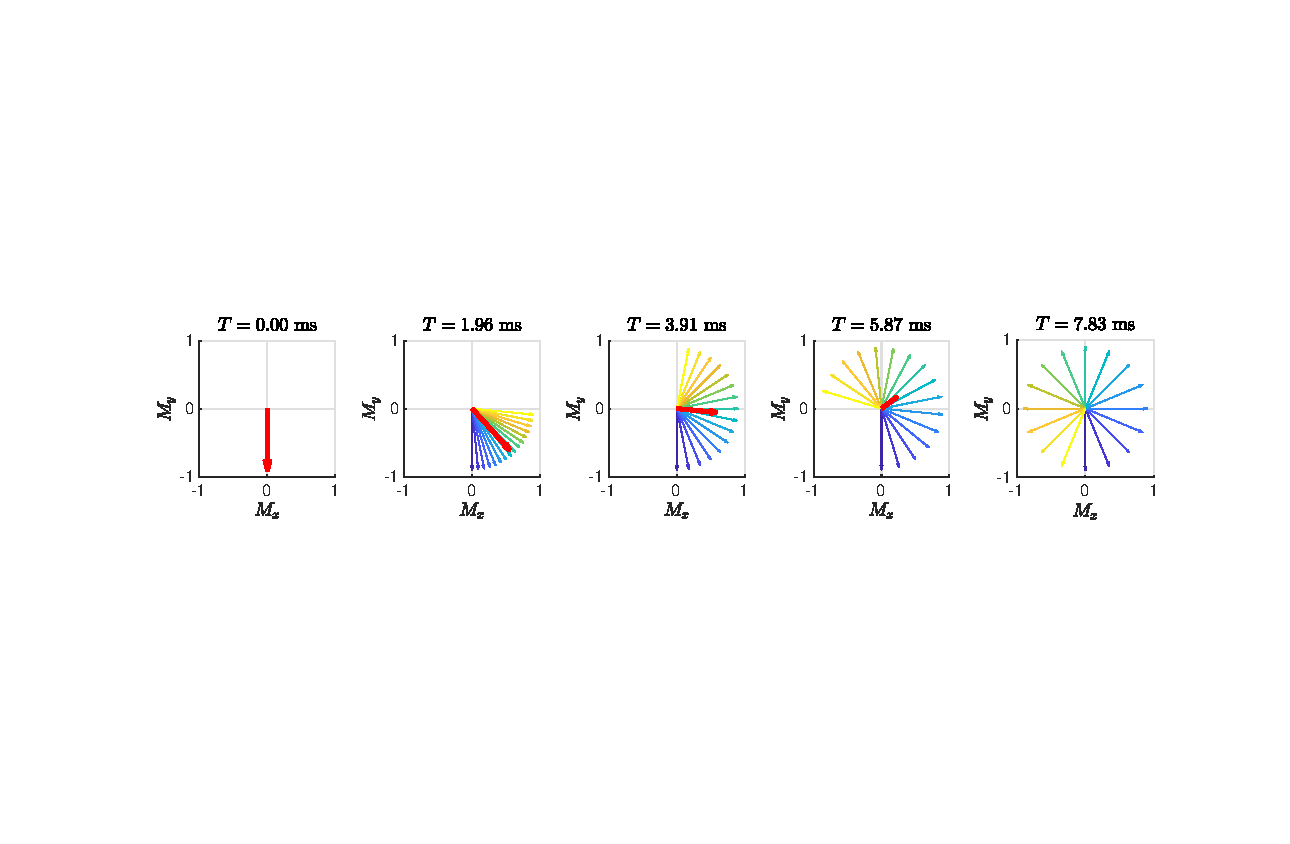
\includegraphics[width=1.0\textwidth]{intraVoxelDephasing.eps}
    \caption{Demonstration of intravoxel dephasing leading to signal decay. From left to right, $T$ is increasing while there is a sub-voxel gradient $G$ present. The blue/yellow arrows represent transverse magnetization at different positions within the voxel. The red arrow is the vector sum of the gray arrows (divided by the number of gray arrows).  }
    \label{fig:ivd}
\end{figure}
\emph{Notice how the vector sum (i.e., the measureable signal) decreases as time goes on}. This causes additional decay on top of $T_2$ decay and is known as $T_2^\prime$ decay. While it cannot always be explicitly represented as exponential decay, the combined effects of $T_2$ and $T_2^\prime$ are often combined into a single time constant $T_2^*$ as:
\begin{equation}
    \frac{1}{T_2^*} = \frac{1}{T_2} + \frac{1}{T_2^\prime}
\end{equation}

\section{Hahn Spin Echoes}

In 1950, American physicist Erwin Hahn first discovered that the effects of $T_2^\prime$ decay were reversible. To mitigate these effects, he used a second RF pulse to reverse the phase of the transverse magnetization. Let's look at the effect of applying a 180-degree RF pulse along the $+x$ direction. 
\begin{equation}
    \mathbf{M}^\prime = 
    \begin{bmatrix}
        1 & 0 & 0\\
        0 & -1 & 0\\
        0 & 0 & -1
    \end{bmatrix}
    \begin{bmatrix}
        M_x\\M_y\\M_z
    \end{bmatrix}
\end{equation}
With these rotations, it is clear that the $M_x$ magnetization component is unchanged by the RF pulse while $M_y$ is negated. Any $M_z$ components gained during $T_1$ recovery between the 90-degree and 180-degree pulses will not contribute the transverse magnetization after the 180 pulse (i.e., because the flip angle is a perfect 180 degrees). 
\begin{figure}[h]
    \centering
    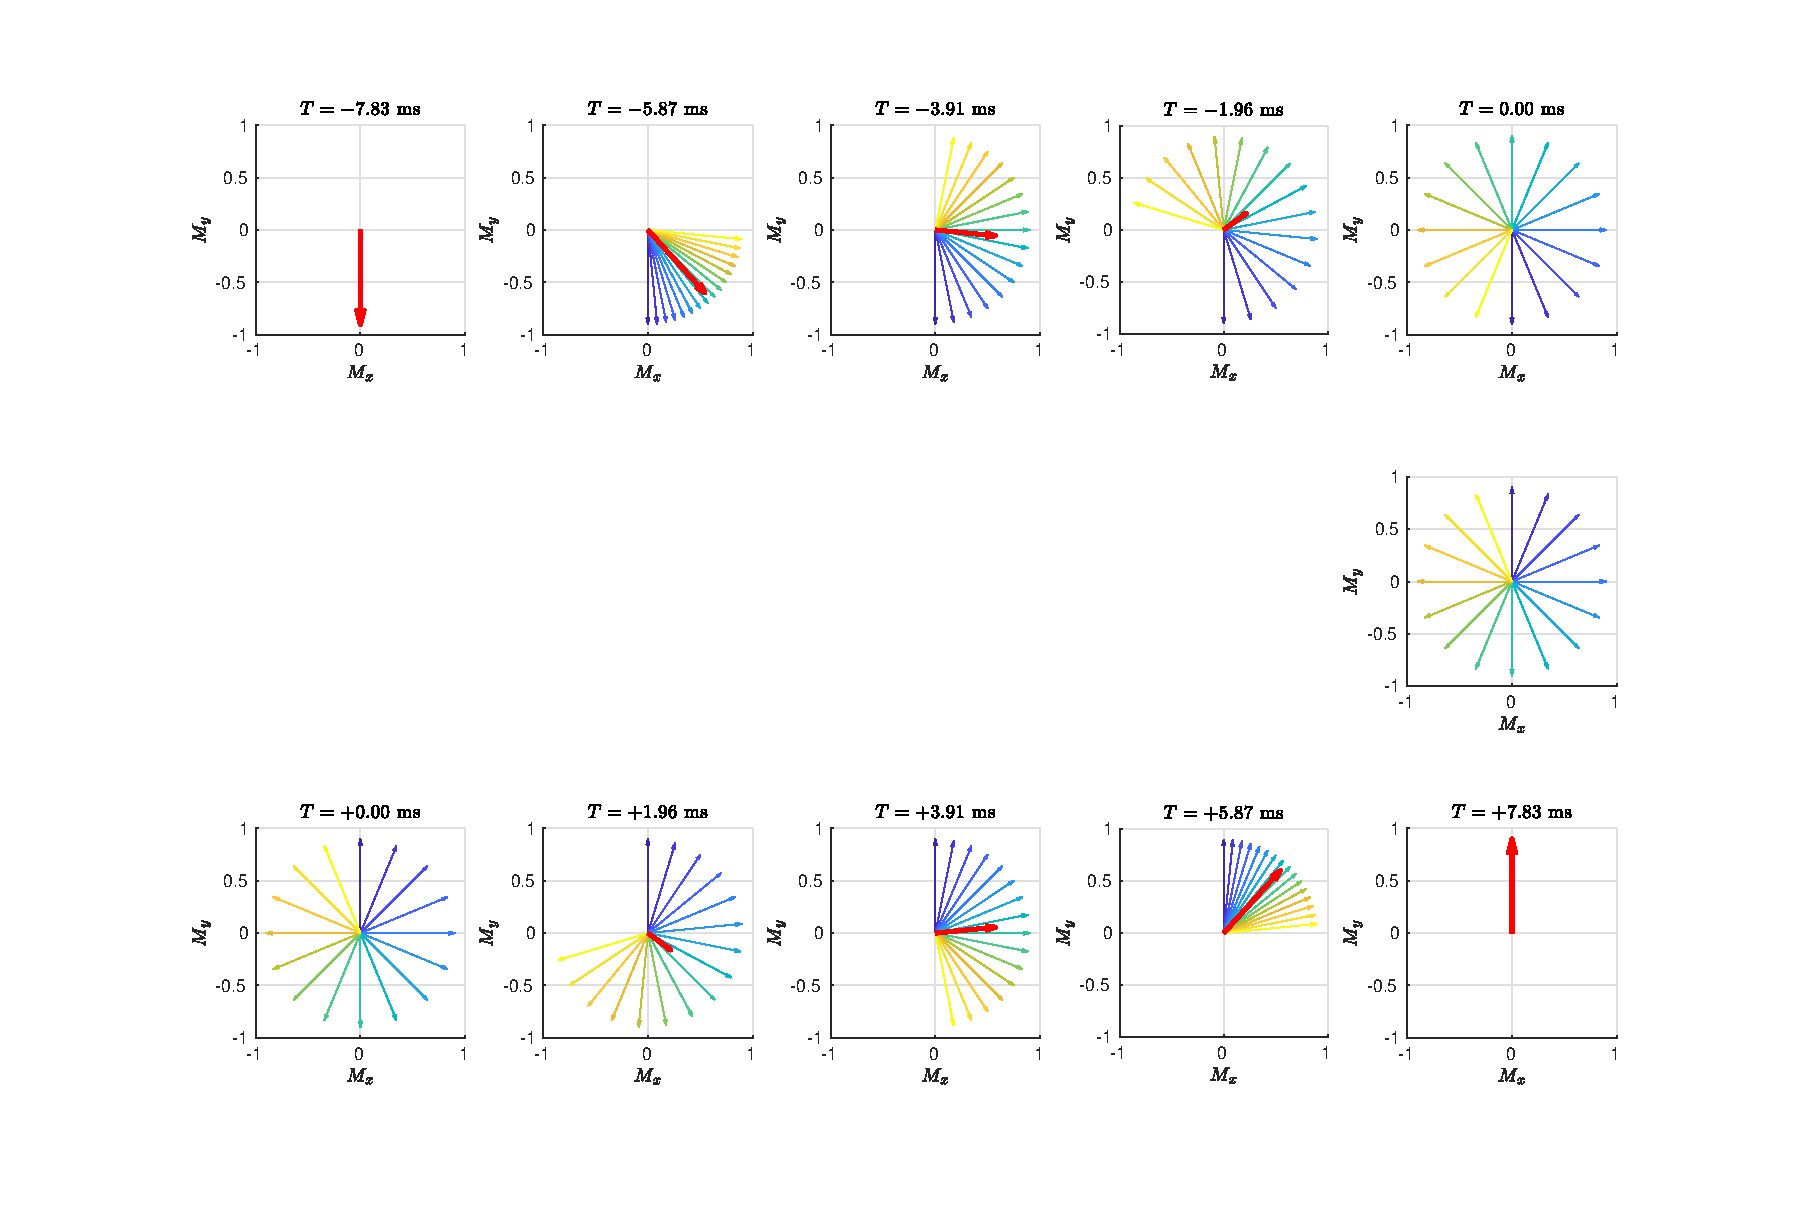
\includegraphics[width=1.0\textwidth]{hahnSpinEcho.eps}
    \caption{Demonstration of Hahn spin echoes to reverse the effects of intra-voxel dephasing leading to $T_2^\prime$ decay. The top row shows the same as Figure 1, just with time periods relative to the 180-degree pulse. The middle row shows that the sign of the $M_y$ component changed as a result of the 180-degree pulse. The bottom row shows that spins are now re-aligning as a result of their different precessional frequencies. }
    \label{fig:ivd}
\end{figure}
With this tool at our disposal, we can measure pure $T_2$-weighted signals without worrying about within-voxel dephasing leading to signal loss. 

\section{Phase Graphs}

While the example above showed how an RF pulse can act as a "refocusing" pulse, every single RF pulse has the potential to do one of three things:
\begin{enumerate}
    \item Take a portion of existing magnetization accumulating phase and continue accumulating phase on that same pathway (i.e., it doesn't change its phase trajectory and continues on the same line).
    \item Act as an excitation pulse, tipping a fraction of longitudinal magnetization into the transverse plane.
    \item Act as a refocusing pulse, taking a fraction of transverse magnetization and changing the sign of its phase. 
    \item Act as a "flip-back" pulse, taking a fraction of transverse magnetization and storing it back along the longitudinal axis. 
\end{enumerate}
The proportions in which each of these actions occur is dependent on the flip angle $\alpha$. Using the complex-valued notation for magnetization (i.e., $[M_x + iM_y\text{, } M_x - iM_y\text{, } M_z]^T$), we can describe what these proportions are calculated to be. Assuming real-valued RF pulses (i.e., only applied along the $x$ direction), these RF pulse effects act on the magnetization as: 
\begin{equation}
    \mathbf{S}\mathbf{R}_x\mathbf{S}^{-1}\mathbf{M} = 
    \begin{bmatrix}
        \cos^2\frac{\alpha}{2} & \sin^2\frac{\alpha}{2} & -i\sin \alpha\\
        \sin^2\frac{\alpha}{2} & \cos^2\frac{\alpha}{2} & i\sin \alpha\\
        \frac{-i}{2}\sin \alpha & \frac{i}{2}\sin \alpha & \cos \alpha
    \end{bmatrix}
    \begin{bmatrix}
        M_x + iM_y\\
        M_x - iM_y\\
        M_z
    \end{bmatrix}
\end{equation}
With this formulation, the complex conjugated magnetization will be the component that is rephasing. 

For a 3-RF-pulse sequence with RF pulses at times $\tau_1=0$, $\tau_2=1\text{ ms}$, and $\tau_3=2.5\text{ ms}$, the phase graph looks as follows. Due to the matrix multiplication with the application of each RF pulse, there are a total of $N^3+1$ pathways, where $N$ is the number of RF pulses. The slope of the phase accumulation must always be positive. Anytime there is a zero-crossing (red marks), a spin echo was produced. In this $N=3$ case, five spin echoes are produced. 

\begin{figure}[h]
    \centering
    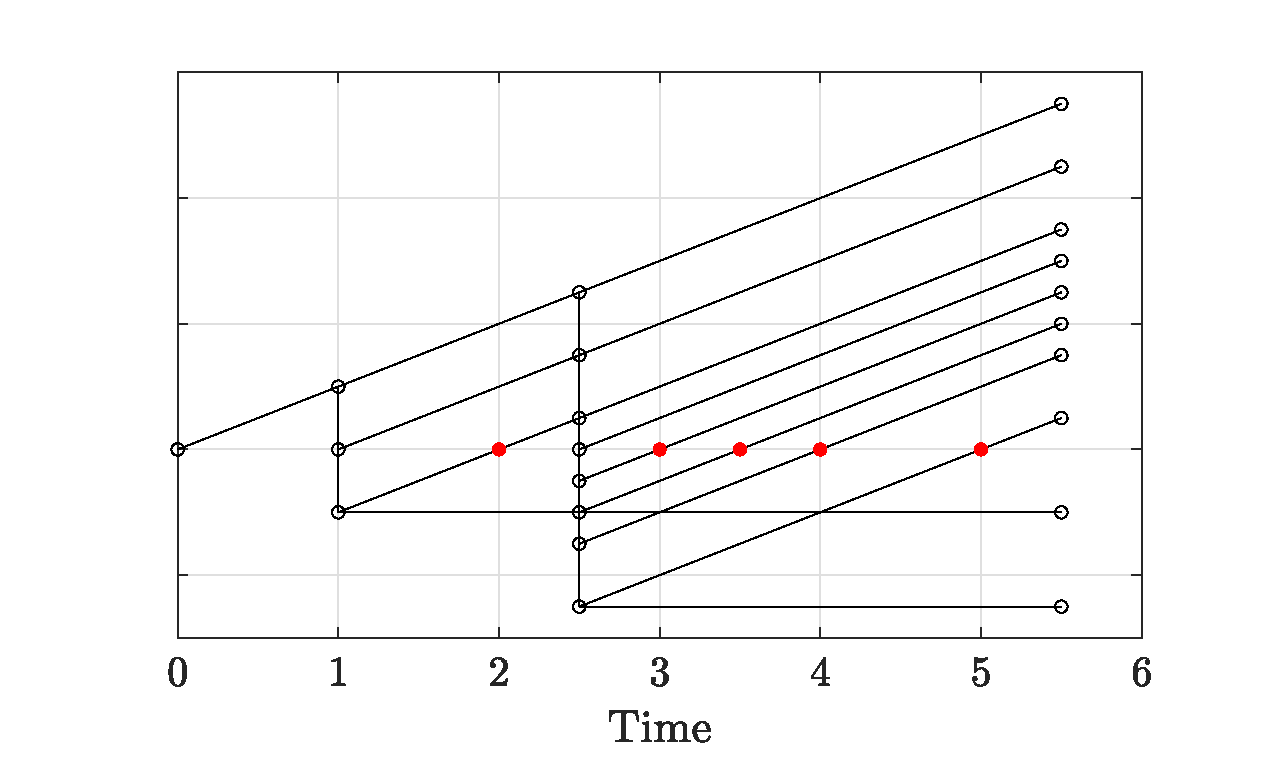
\includegraphics[width=1.0\textwidth]{phaseGraph3RF.eps}
    \caption{Phase graph for three RF pulses occurring at $\tau_1=0$, $\tau_2=1\text{ ms}$, and $\tau_3=2.5\text{ ms}$.}
    \label{fig:ivd}
\end{figure}

\begin{figure}[h]
    \centering
    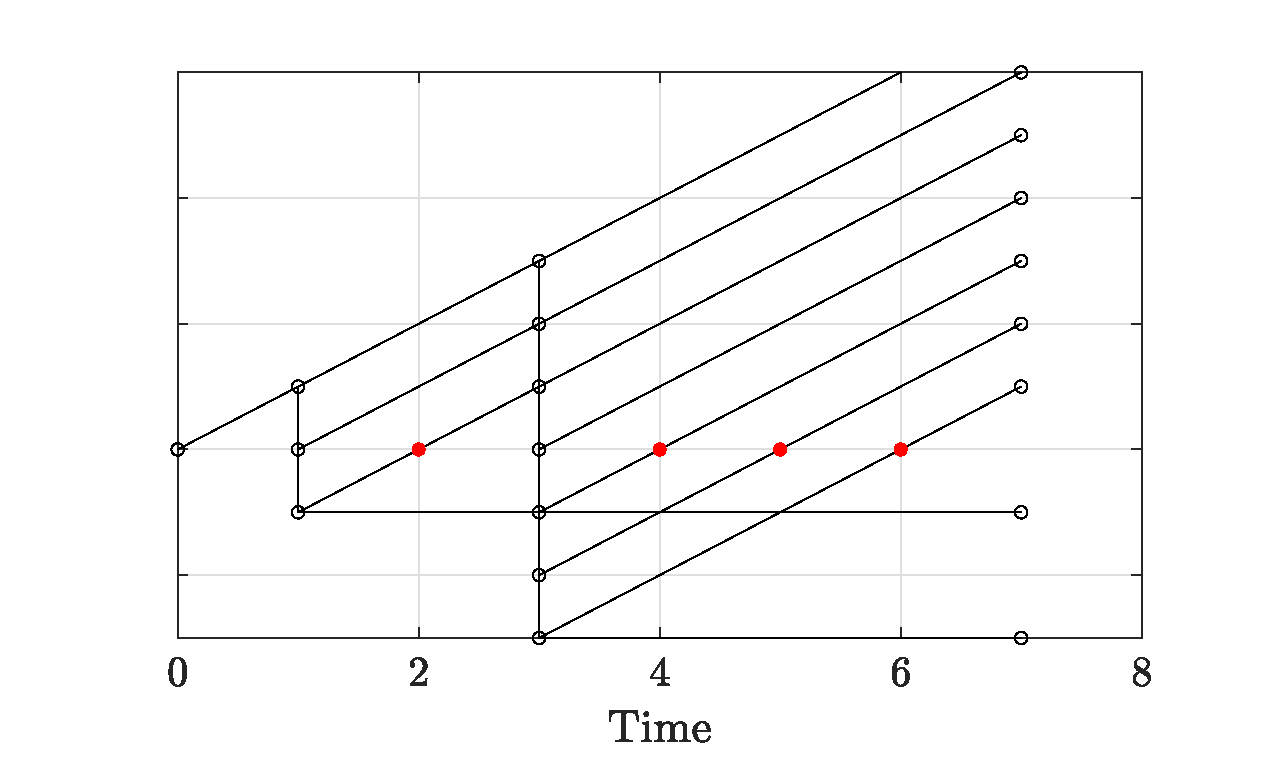
\includegraphics[width=1.0\textwidth]{phaseGraphCPMGTiming.eps}
    \caption{Phase graph for three RF pulses occurring at $\tau_1=0$, $\tau_2=1\text{ ms}$, and $\tau_3=3\text{ ms}$. Note that two of the echoes now occur at the exact same time of 4 ms.}
    \label{fig:ivd}
\end{figure}

\section{Using Gradients to Eliminate Unwanted RF Pathways}

As seen in Figure 1, a measurable signal within a voxel will be canceled if there is a phase dispersion of $2\pi$ between spins resonating at different frequencies. In spin MRI, it is often desired to \emph{intentionally} dephase spins within a voxel to eliminate one or components of its signal. For example, it may be desirable to eliminate one of the echoes occurring simultaneously at time $t=4$ in Figure 4. To intentionally dephase the magnetization within a voxel, we can use the imaging gradients to achieve a phase of $n \cdot 2 \pi$ across the voxel with $n$ being any integer greater than zero (with a typical value being $n=2$ or $n=4$. Let's say our voxel is oriented along the $x$ axis with a dimension $\Delta x$. The $G_x$ gradient with duration $T_G$ is calculated to ensure a proper dephasing as follows: 
\begin{equation}
    \Delta x \gamma \int_0^{T_G} G_x(t) dt = n \cdot 2\pi
\end{equation}

The most common use of these dephasing (or so-called "crusher") gradients are to eliminate the free induction decay occurring after a second RF pulse intended to act as a refocusing pulse. A 2D spin echo pulse sequence can be seen with and without these crusher gradients below. 
\begin{figure}[h]
    \centering
    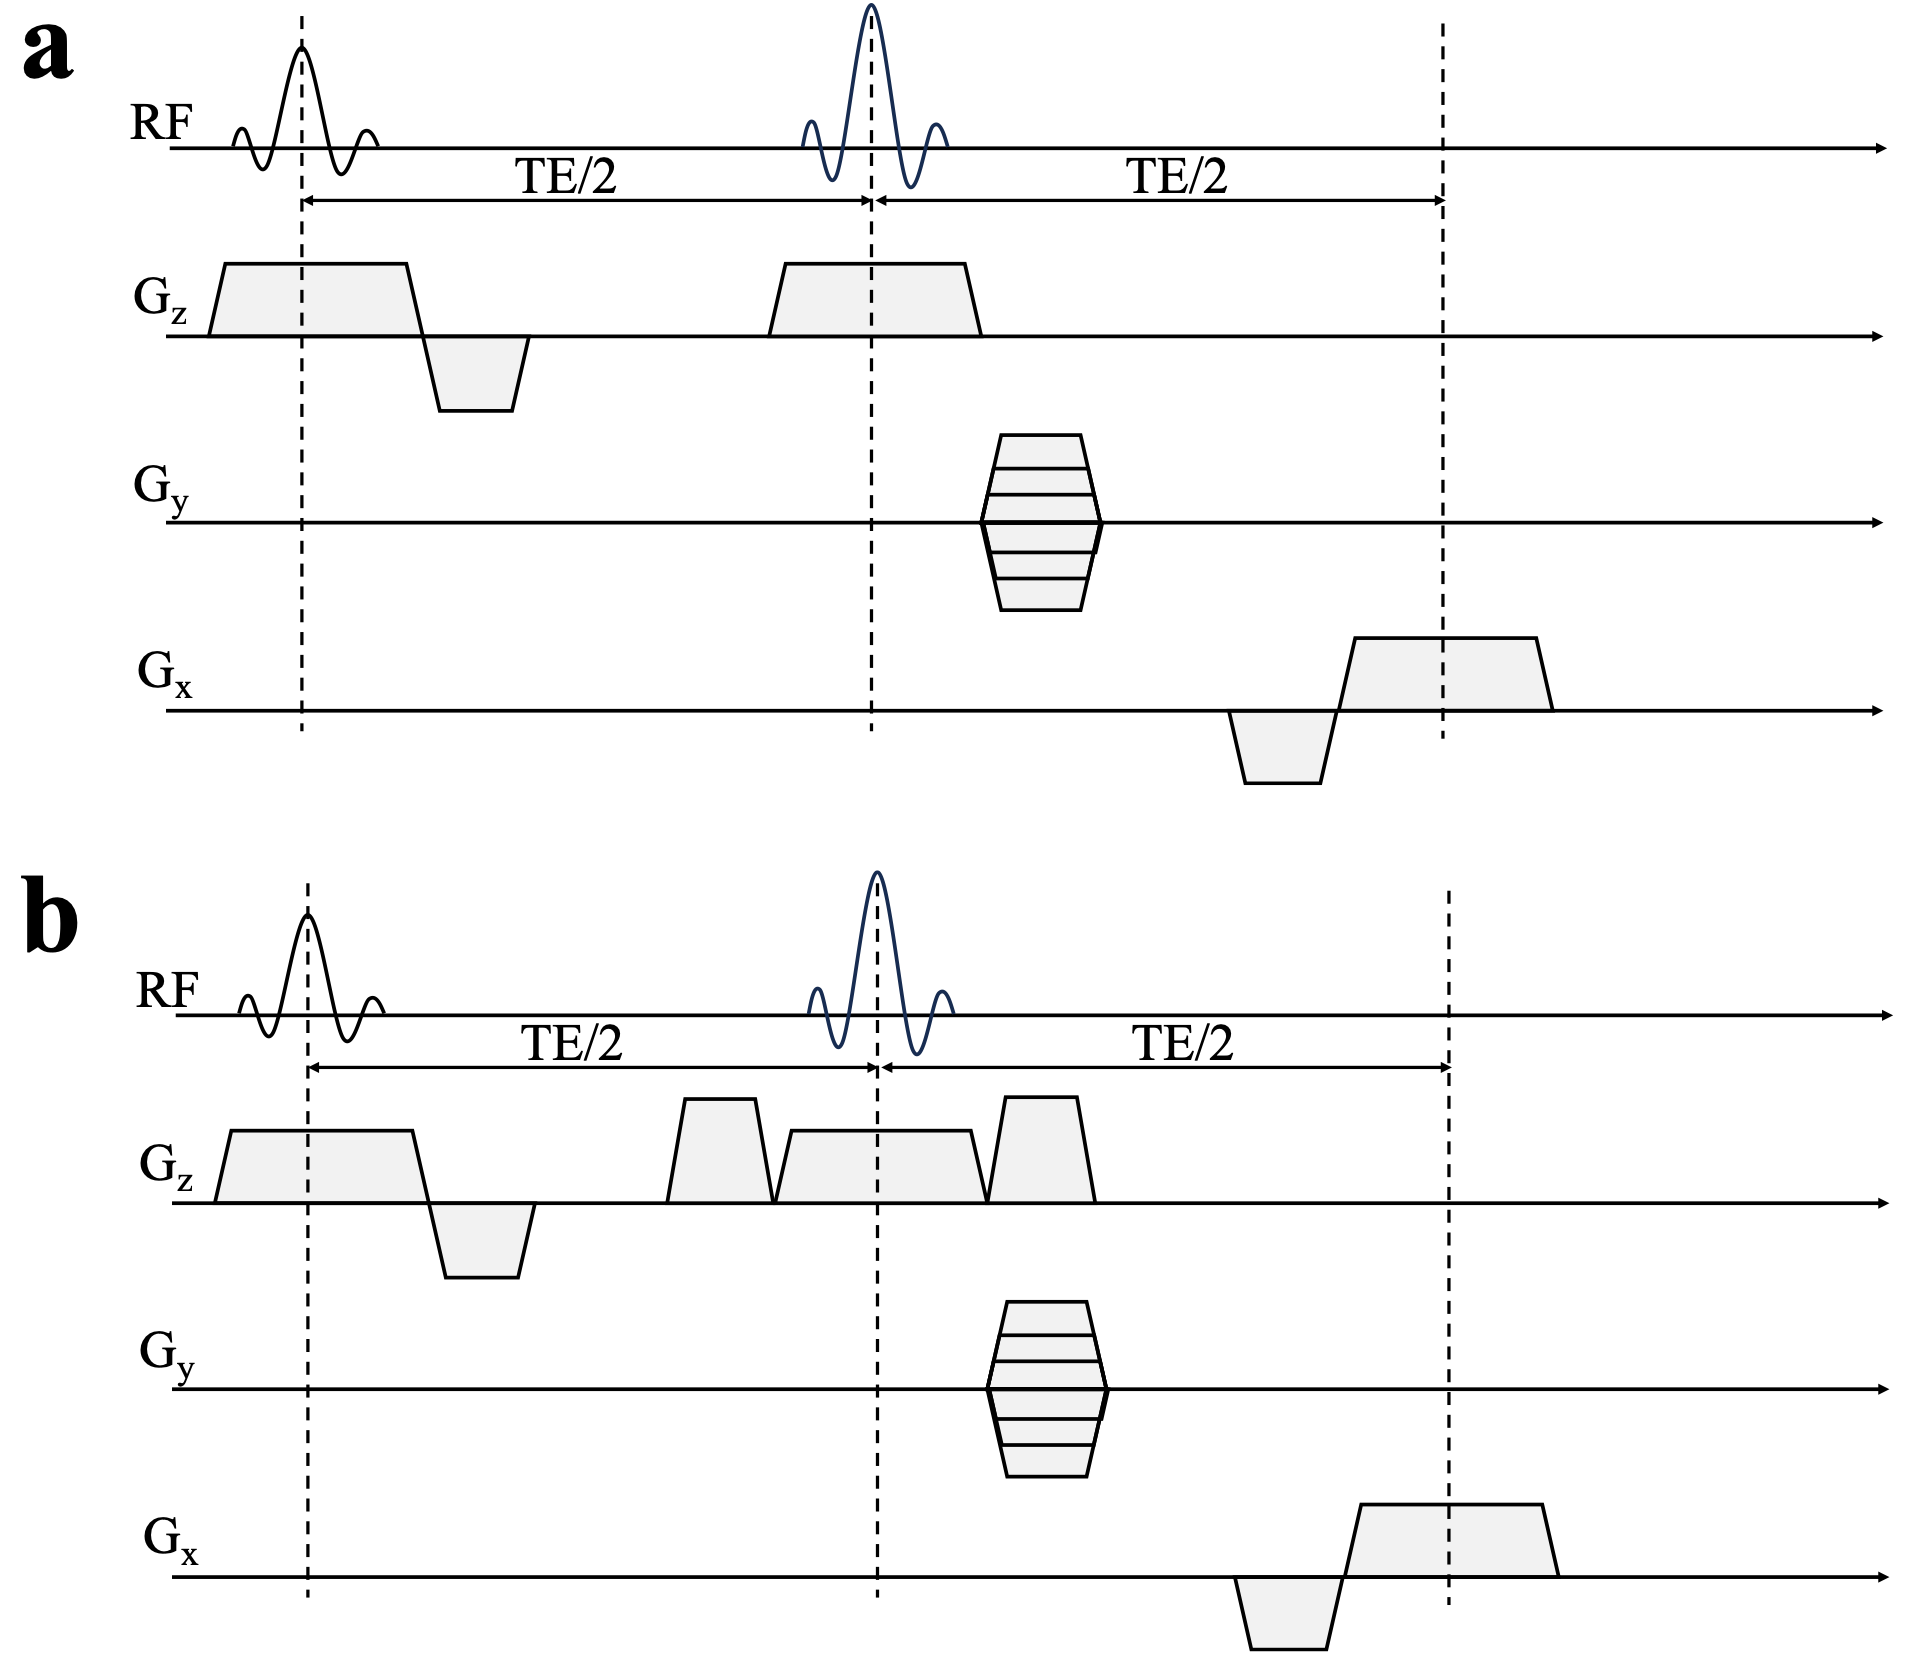
\includegraphics[width=0.75\textwidth]{spin_echo_crushers.png}
    \caption{a) 2D spin echo pulse sequence with a spin echo occurring at the echo time (TE). b) The same 2D spin echo pulse sequence with crusher gradients to eliminate free induction decay. }
    \label{fig:ivd}
\end{figure}

As seen in Figure 2, in order for a spin echo to form, the exact amount of phase that accumulated before the application of the refocusing pulse must also accumulate after the refocusing pulse. So, even though we only want to dephase the FID occurring after the second RF pulse, we have to also add a crusher gradient \emph{before} the second refocusing pulse to ensure the spin echo will still form. 

\section{Making Spin Echo Imaging Faster}

Repeating the pulse sequence in Figure 5 for each phase encoding line is time consuming. Luckily, we can use what is known as a "fast spin echo" pulse sequence to acquire several lines of k-space after a single excitation, each line occurring along with a new spin echo. The pulse sequence is shown below:
\begin{figure}[h]
    \centering
    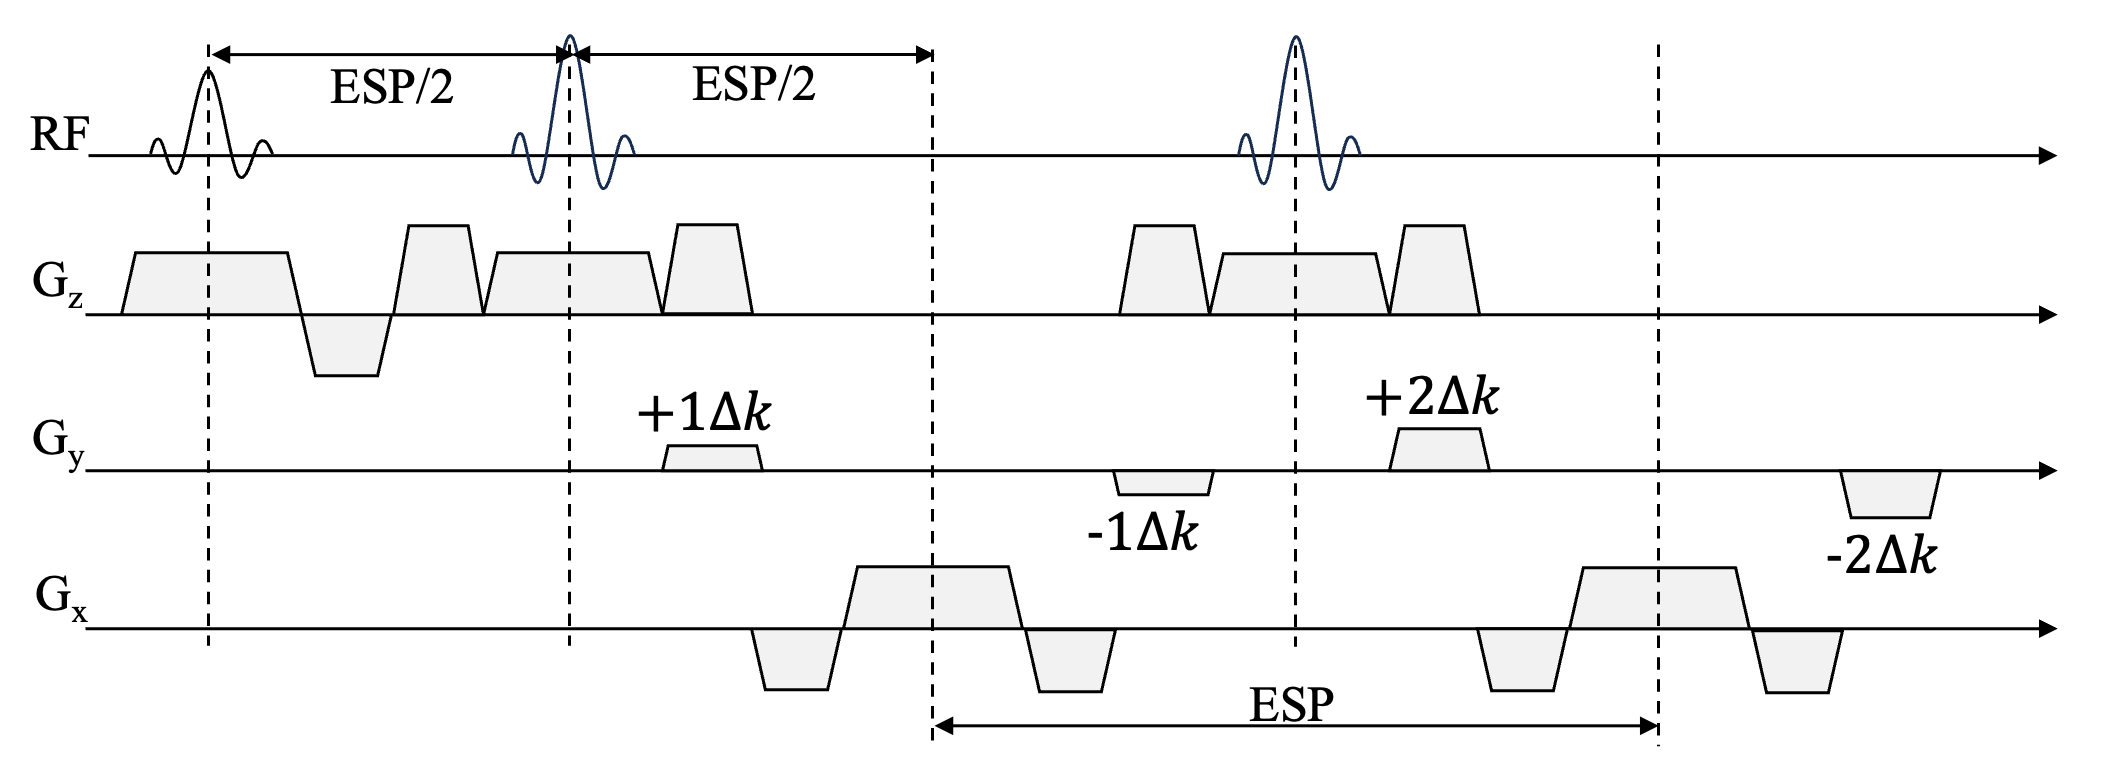
\includegraphics[width=0.75\textwidth]{fse.png}
    \caption{2D fast spin echo imaging pulse sequence diagram. }
    \label{fig:ivd}
\end{figure}

There are a few things to note with this pulse sequence. First, the timing is now parameterized by the "echo spacing" (ESP), which is the time between consecutively formed spin echoes. Second, this sequence can continue on in time. While I have only shown two refocusing pulses to collect two phase encoding lines, you can use, for example 16 refocusing pulses to collect 16 lines in $k$-space. Third, you will notice that the gradients along the $x$ and $y$ axis are slightly different than in Figure 5. This is because it is important that the phase accumulated between any two consecutive refocusing pulses must be constant. Therefore, the phase accumulated from the phase encoding and frequency encoding processes is "rewound" back to zero after the data are collected. The timing and rewinding of phase are characteristics known as the Carr-Purcell-Meiboom-Gill (CPMG) conditions. 

There is never a free lunch in MRI, and fast spin echo imaging, while allowing for more efficient collection of $k$-space samples, introduces new artifacts. These artifacts arise from the fact that $k$-space samples are acquired \emph{while $T_2$ decay is occurring.} This has the effect of applying a filter that changes exponentially as a function of $k$-space. The impact his has on the fidelity of an image can be seen in the 1D simulation in Figure 7.
\begin{figure}[h]
    \centering
    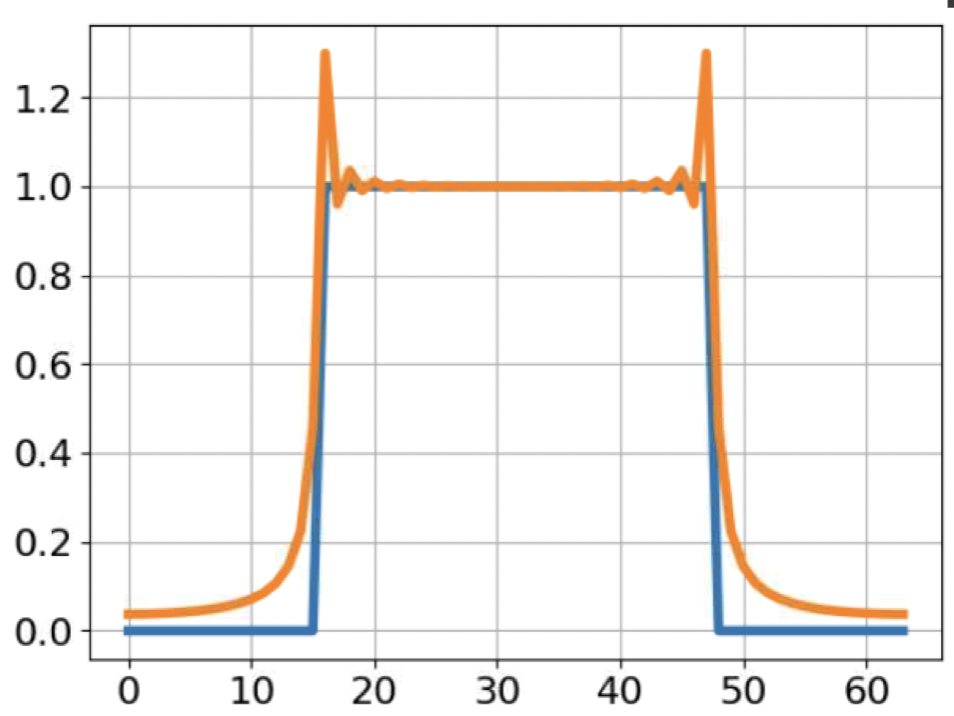
\includegraphics[width=0.5\textwidth]{fse_blur.png}
    \caption{FSE $k$-space signal was simulated for an ideal 1D object (blue) and reconstructed (orange) to show the impact of the exponential filter seen in $k$-space due to $T_2$ decay. The result is blurred edges and ringing due to the asymmetric amplitudes of high spatial frequency components.  }
    \label{fig:ivd}
\end{figure}

The loss of resolution is an important consideration when determining the appropriate pulse sequence for a given application; And, if a fast spin echo sequence is selected, parameters such as the echo spacing and echo train length must be carefully selected. 

\begin{equation}
    \cos^2(\alpha_3/2) \Big( -i M_0 \sin(\alpha_1) \cos^2(\alpha_2/2) + i M_0 \sin(\alpha_1) \sin^2(\alpha_2/2) - i M_0 \sin(\alpha_2) \cos(\alpha_1) \Big) + \sin^2(\alpha_3/2) \Big( -i M_0 \sin(\alpha_1) \sin^2(\alpha_2/2) + i M_0 \sin(\alpha_1) \cos^2(\alpha_2/2) + i M_0 \sin(\alpha_2) \cos(\alpha_1) \Big) - i \sin(\alpha_3) \Big( -M_0 \sin(\alpha_1) \sin(\alpha_2) + M_0 \cos(\alpha_1) \cos(\alpha_2) \Big)
\end{equation}

\end{document}